%%% Laboratory	 Notes
%%% Template by Mikhail Klassen, April 2013
%%% Contributions from Sarah Mount, May 2014
\documentclass[a4paper]{tufte-handout}

\newcommand{\workingDate}{\textsc{May $|$ 2014}}
\newcommand{\userName}{Your Name}
\newcommand{\institution}{Your University}

\usepackage{lab_notes}
\usepackage{listings}

\usepackage{hyperref}
\hypersetup{
  pdffitwindow=false,            % window fit to page
  pdfstartview={Fit},            % fits width of page to window
  pdftitle={Lab notes 2014},     % document title
  pdfauthor={Your Name},         % author name
  pdfsubject={},                 % document topic(s)
  pdfnewwindow=true,             % links in new window
  colorlinks=true,               % coloured links, not boxed
  linkcolor=DarkScarletRed,      % colour of internal links
  citecolor=DarkChameleon,       % colour of links to bibliography
  filecolor=DarkPlum,            % colour of file links
  urlcolor=DarkSkyBlue           % colour of external links
}


\title{BB Training Notes}
\date{2017}

\begin{document}
\maketitle

\newday{23 July 2017}
Chaper 1
\begin{projects}
  Symbol Table
  \begin{itemize}
  \item it is a data structure maintained by compiler
  \item store names of all entities
  \item verify if a veriable has been declared
  \item determine the scope of a name
  \item used to realize type checking
  \end{itemize}

  \begin{itemize}
  \item Declaration introduces the name and type of a variable so that the compiler knows what the name means if it occurs later in the program.
  \item Variable Definition causes the compiler to reserve a memory block of appropriate size to hold the value of the variable.
  \end{itemize}

  Declaration and Definition
  \begin{lstlisting}[language=C]
    int a;//definition and declaration
    extern int a;//declaration
    int b = 1;//definition and declaration
  \end{lstlisting}
\end{projects}

Constants
\begin{enumerate}
\item Constants are variables that value never change. They are called immutable.
\item As a convention, always name constants with UPPER\_SNAKE\_CASE;
\end{enumerate}

Naming Convention
\begin{itemize}
\item Camel case: words seperated by initial capital letter (camelCase or CamelCase).
\item Snake case: words seperated by underscore (snake\_case or SNAKE\_CASE).
\item Variable and functions: camel case with lower case first letter. avgInvest...
\item Constancs: all captial snake case.
\item Type and class: camel case with uppercase first letter. StockContainer...
\end{itemize}

Operator
\begin{itemize}
\item Discuss that the assignment operator yields as a value the value being assigned, but the main purpose is the side-effect that a the value is assigned to the variable.
\item Discuss that for <<, the main purpose is the side effect (i.e., inserting the data into the stream). And yes, it yields a stream as a value that is needed for chaining.
  \begin{lstlisting}[language=C]
    if(a = 0)...//false
    if(a = 1)...//true
  \end{lstlisting}
\item Caution! If all the operands are integers then integer division is performed, any fractional part is automatically discarded!
  \begin{lstlisting}[language=C]
    double tempF = tempC * 9 / 5 + 32;//loss precision
    double tempF = tempC * 9.0 / 5 + 32;//accurate
  \end{lstlisting}
  \begin{lstlisting}[language=c]
    bsl::cout << ``Hello'' << name << ``\n'';
    effectively is (((bsl::cout << ``Hello'' ) << name) << ``\n'');
    Explain that a = b = c= 123;
    is the same as a = ( b = ( c = 123; ) )
  \end{lstlisting}
  This introduces an example of an operator that is right associative.Also, this explain why an assignment returns bthe value that it assigns.
\end{itemize}

Basic input and output

\begin{enumerate}
\item C++ uses streams to abstract input and output
  Streams can represent the screen, keyboard, a file, etc.
\item Streams are used to either insert or extract characters
  They represent a source or destination
  Characters are handled sequentially, one after the other
\item bsl::endl is a stream manipulator that inserts a newline character
  \begin{itemize}
  \item But also requests the data is physically written to the destination (called flushing).
  \item Flushing is usually expensive and streams have optimisations to minimise it
  \end{itemize}
\item
\end{enumerate}

%%%%%%%%%%%%%%%%%%%%%%%%%%%%%%%%%%%%%%%%%%%%%%%%%%%%%%%%
\newday{July 26th 2017}
Bash

command + \& -> run in background \newline
shell define vaiable without \$, access variable with \$.
quote stop match regular expression but does not stop variable access.

Vim\newline
x - delete char\newline
5x - delete 5 chars\newline
dd - delete a whole line \newline
5dd - delete 5 lines \newline
dw - delete a word \newline
5dw - delete 5 words \newline
shift + char - capital char (also valid in Emacs) \newline
cw - change word \newline
. - repeat last command \newline
cc - change the entire line \newline
\$ end of line, \^ beginning of line \newline
:+10 :-5 move cursor according to line number \newline

C++\newline
main can't be put in a namespace or the compiler won't find it because it won't be main in the symbol table but with some extra prefix related with the namespace.\newline
a() + b() + c(), specific evaluation sequence is not defined before C++11.\newline
reference much be initialized, pointer could point to null.
%%%%%%%%%%%%%%%%%%%%%%%%%%%%%%%%%%%%%%%%%%%%%%%%%%%%%%%%
\newday{July 27th 2017}

\textbf{GIT}
\begin{enumerate}
\item The stage is used for telling Git what to care about in future commands.
\item To remove files from stage : git reset  HEAD [path] e.g.\ git reset HEAD readme.md
\item Commit creat a snapshot in history of all files
\item Supplies a unique hash used for referring to the moment in histroy
\item To keep files but remove Git tracking : git rm --cached [file]
  \begin{itemize}
  \item --cached tells Git to remove tracking on this file, but keep local file.
  \item git rm [file] remove local
  \end{itemize}
\item A fork creates a remote repository by cloning
\item Use pull request to merge changes in fork back to its parent repository.
\item Note that each commit hash actually reference a complete snapshot of the repository. The snapshot contains a commit hash for EVERY FILE.
\item remote remote branch git push origin :{branch-name} \footnote {Pay attention to the space positon}
\item Fast forward merg happen only if history has not diverged
  \item merge order, merge master on current branch, checkout to master and merge local feature branch, push master, delete local branch
\end{enumerate}
\begin{maybe}
  \begin{itemize}
  \item Reimplement the ideas from the paper \textit{Getting Reference Counting Back in the Ring} \citep{Shahriyar+12}
  \end{itemize}
\end{maybe}

%%%%%%%%%%%%%%%%%%%%%%%%%%%%%%%%%%%%%%%%%%%%%%%%%%%%%%%%

\newday{10 June 2014}

The (very fast) OCaml to Javascript compiler described in \citep{VouillonBalat13}\footnote{\url{http://ocsigen.org/js_of_ocaml/}} takes the unusual approach of compiling OCaml \textit{bytecode} to Javascript, rather than performing a source-to-source translation.

\hrulefill

%%%%%%%%%%%%%%%%%%%%%%%%%%%%%%%%%%%%%%%%%%%%%%%%%%%%%%%%

\newday{9 June 2014}

Poor benchmark results. Ideas for improvement are listed in the issue tracker in the repository.

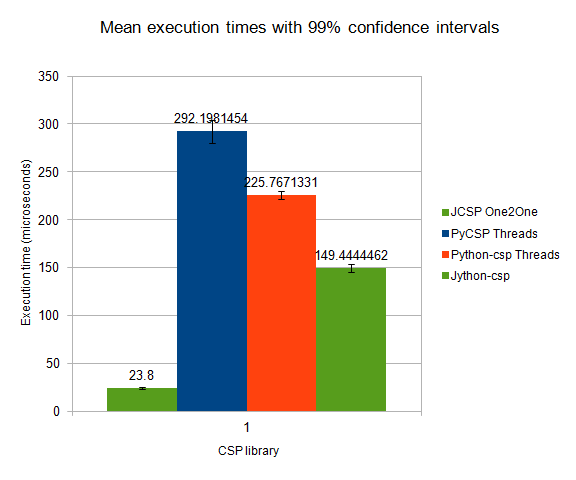
\includegraphics[scale=0.65]{benchmark}

\hrulefill

%%%%%%%%%%%%%%%%%%%%%%%%%%%%%%%%%%%%%%%%%%%%%%%%%%%%%%%%

\newday{6 June 2014}
Discuss that for <<, the main purpose is the side effect (i.e., inserting the data into the stream). And yes, it yields a stream as a value that is needed for chaining.

Back from vacation.

\newthought{Student project idea} improve \url{https://github.com/snim2/Terminus} by adding new BASH commands.

Size of data sets for the ngram paper are shown in Table \ref{tab:ngram-sizes}.

\begin{table}[p]
  \label{tab:ngram-sizes}
  \centering
  \caption{Data sizes in Google ngram data}
  \begin{tabular}{lrr}
    \toprule
    Data 	&	Rows &	Compressed Size (GB)\\
    \midrule
    English\\
    \midrule
    1 gram &	472,764,897 &	4.8\\
    2 gram &	6,626,604,215 &	65.6\\
    3 gram &	23,260,642,968 &	218.1\\
    4 gram &	32,262,967,656 &	293.5\\
    5 gram &	24,492,478,978 &	221.5\\
    \textbf{Totals} &	87,115,458,714 &	803.5\\
    \midrule
    English One Million\\
    \midrule
    1 gram &	261,823,186 &	2.6\\
    2 gram &	3,383,379,445 &	32.1\\
    3 gram &	10,565,828,499 &	94.8\\
    4 gram &	12,987,703,773 &	113.1\\
    5 gram &	8,747,884,729 &	75.8\\
    \textbf{Totals} &	35,946,619,632 &	318.4\\
    \midrule
    American English\\
    \midrule
    1 gram &	291,639,822 &	3\\
    2 gram &	3,923,370,881 &	38.3\\
    3 gram &	12,368,376,963 &	113.9\\
    4 gram &	15,118,570,841 &	135\\
    5 gram &	10,175,161,944 &	90.2\\
    \textbf{Totals} &	41,877,120,451 &	380.4\\
    \midrule
    British English\\
    \midrule
    1 gram &	188,660,459 &	1.9\\
    2 gram &	2,000,106,933 &	19.1\\
    3 gram &	5,186,054,851 &	46.8\\
    4 gram &	5,325,077,699 &	46.6\\
    5 gram &	3,044,234,000 &	26.4\\
    \textbf{Totals} &	15,744,133,942 &	140.8\\
    \midrule
    English Fiction\\
    \midrule
    1 gram	&	191,545,012	&	2\\
    2 gram	&	2,516,249,717	&	24.3\\
    3 gram	&	7,444,565,856	&	68\\
    4 gram	&	8,913,702,898	&	79.1\\
    5 gram	&	6,282,045,487	&	55.5\\
    \textbf{Totals}	& 25,348,108,970	&	228.9\\
    \midrule
    \textbf{Total without 1M}  &	170,084,822,077 &	1553.6\\
    \textbf{Total without 1M} &  &	1.53TB\\
    \textbf{Total}	& 206,031,441,709 &	1872\\
    \textbf{Total}	& &	1.848TB\\
  \end{tabular}
\end{table}


\hrulefill

%%%%%%%%%%%%%%%%%%%%%%%%%%%%%%%%%%%%%%%%%%%%%%%%%%%%%%%%

\newday{May 30 2014}

Useful datasets: \url{http://rs.io/2014/05/29/list-of-data-sets.html} In particular Mozilla have released a defect tracking dataset on GitHub\footnote{\url{https://github.com/ansymo/msr2013-bug_dataset}}\citep{Lamkanfi+13}.

Google NGram dataset can be found in Amazon S3\footnote{\url{http://aws.amazon.com/datasets/8172056142375670}}.

\hrulefill

%%%%%%%%%%%%%%%%%%%%%%%%%%%%%%%%%%%%%%%%%%%%%%%%%%%%%%%%

\newday{Jan 20 2013}

\textit{N.B.: The following is a sample entry from Mikhail Klassen's research diary. It is intended to be illustrative of how WriteLaTeX can be used the keep track of your research progress. Some names have been removed from this document for privacy.}

\section*{Initial conditions for the turbulent molecular cloud run}

\subsection*{Inner radius}

The density profile follows an $r^{-3/2}$ power law. To avoid a singularity at the center, an interpolation is done over a radius. This inner radius is defined in the parameter file. It should follow the prescription of a singular isothermal sphere (see Binney \& Tremaine p.305), which is also the definition of the King radius:
\begin{equation}
  r_0 \equiv \sqrt{\frac{9\sigma^2}{4\pi G\rho_0}}
\end{equation}
where $\sigma$ is the velocity dispersion and could be estimated as $\sigma = \mathcal{M} c_s$, where $c_s = \sqrt{\gamma P/\rho} = \sqrt{\gamma k_B T / \mu}$ is the sound speed.

The isothermal sound speed in our simulation was estimated
\begin{equation}
  c_s = \sqrt{\frac{k_b T}{\mu m_p}}
\end{equation}
I'm unsure why a factor of $\gamma$ was not included. For 30 K, this gives a sound speed of about 34000 cm/s or 0.34 km/s. At a Mach number of 5, this gives a supersonic dispersion of $\sigma$ = 1.7 km/s

This gives an inner radius of $r_0 \approx$ 1.595e17.

\subsection*{Rotation}

Set the same ratio of rotational to gravitational energy $\beta$ as in Peters et al. 2010a. According to Goodman et al. (1993), this is given by (see equation 6):
\begin{equation}
  \beta = \frac{1}{4 \pi G \rho_0} \omega^2
\end{equation}
In practice we can probably use the central density $\rho_c$ instead of determining an average density $\rho_0$. Looking at the numbers from other simulations, we could use an $\omega$ of 1.3e-14.

The link to the Goodman et al. (1993) paper:\\
{\tt http://adsabs.harvard.edu/cgi-bin/bib\_query?1993ApJ...406..528G}

We want to complete our simulation with a similar $\beta$ to check if disks form in the turbulent environment.

The $\omega$ necessary to produce a $\beta = 0.05$ would be
\begin{equation}
  \omega = \sqrt{4 \pi G \rho_0 \beta} \approx 7.15\times 10^{-13}
\end{equation}
using $\rho_0 = \rho_c = 1.22\times10^{-17}$.

After testing this, however, I found that the rotation was much too fast. Perhaps using $\rho_0 = \rho_c$ was not a very good assumption at all, since $\rho_c$ is orders of magnitude larger than the average. I wrote a little Python script that sums up all the mass inside the outer radius and divides it by the total volume, defined by the outer radius. In this case, for an outer radius of $5.97402\times 10^{18}$ cm and about 1000 $\Msun$, we get an average density of $2.96415\times 10^{-21}$ g/cm$^3$, which gives us $\omega = 1.114 \times 10^{-14}$.

%\hrulefill

%%%%%%%%%%%%%%%%%%%%%%%%%%%%%%%%%%%%%%%%%%%%%%%%%%%%%%%%

%\newpage
\bibliographystyle{plain}
\bibliography{lab_notes}

\end{document}
